\documentclass[12pt,letterpaper]{article}
\usepackage{geometry}
\usepackage[utf8]{inputenc}
\usepackage{natbib}
\usepackage{lscape}
\usepackage{amsmath}
\usepackage{amsfonts}
\usepackage{amssymb}
\usepackage{graphicx}
\usepackage{subfig}
\usepackage{float}
\usepackage{algpseudocode}
\usepackage{fancyhdr}
\usepackage{comment}
\usepackage{hyperref}

\usepackage[english]{babel}
\geometry{verbose,letterpaper,tmargin=3cm,bmargin=3cm,lmargin=2.5cm,rmargin=2.5cm}

% Tables
\usepackage{multirow}
\usepackage[table]{xcolor}

% Avoid to split words at the end of each line
\usepackage[none]{hyphenat}

\usepackage{setspace}

\usepackage{natbib} 
\setcitestyle{numbers,square}

\usepackage{notoccite}


\singlespacing

\begin{document}

% BEGIN TITLE PAGE
\begin{titlepage}

\Large
\sffamily

\begin{center}
  \begin{tabular}{c}
    
\includegraphics[width=0.30\textwidth]{logo-eafit.png}
  \end{tabular}
\end{center}

\vfill
\begin{center}
  \LARGE Title
\end{center}

\vspace*{1cm}
\centerline{\LARGE Alejandro Salazar Arango\footnotemark}  
\footnotetext{Student information (\textcolor{red}{email})}
\vfill

\begin{center}
Advisor(s): \\
Cristhian David Zambrano Mora\footnote{Affiliation, \textcolor{red}{email}}   \\
\end{center}

\vfill

\begin{center}
  \large
    Research practice 3 \\
  Research proposal \\
  Mathematical Engineering\\
  School of Applied Sciences and Engineering\\
  Universidad EAFIT \\
\end{center}

\vfill
\centerline{August 2023}
\vspace*{0.7cm}
\end{titlepage}

% END TITLE PAGE

\section{Introduction}

\begin{comment}

  (\textcolor{red}{4 a 5 párrafos})

Debe incluir:

\begin{itemize}
\item Contexto corto para ubicar al lector.
\item Corta descripción del problema u oportunidad de investigación.
\item Aporte de la investigación.
\item Párrafo que justifique la importancia de la investigación.
\end{itemize}

\end{comment}


The brain is by far the most metabolically active organ in the human body, 
accounting for about $25\%$ of the total metabolic activity of a person
while being only around $2.5\%$ of his/her total weight \cite{Ischemia}.
This is why the brain is also one of the most sensitive organs to decreases 
in the supply of oxygen delivered to it and therefore has the most complex 
circulatory self-regulation system of the body,  having multiple mechanisms 
to keep the blood flow as stable as possible and to compensate for the 
oscillations caused by body processes \cite{AnatoFisio}. When these normal
levels of blood flow are compromised,  ischemia,  or in more general terms, 
a stroke is caused.\\~\\
A stroke is a medical condition where brain cells die due to oxygen starvation,
originated from a disruption in the blood supply to the brain. It can
be classified into two main types, hemorrhagic, when the cause is internal bleeding
on the brain and ischemic when it is caused by the lack of blood flow,  being the 
latter the most common,  accounting for $87\%$ of all strokes \cite{johns_hopkins_medicine}.
They are considered one of the leading causes of death and a major cause
of disability worldwide. In 2019 Stroke's global prevalence was 101.5 million 
people,  of which 6.6 million were fatal \cite{burden},  and even though this shows 
a decrease in the number of incidents in comparison to previous years,  Strokes keep being a
matter of concern for the medical scientific community.\\~\\
It’s because of this and because of many other reasons that in recent years 
not only the medical community,  but the scientific community in general,  
has focused great efforts on blood flow analysis,  and this is where computational 
fluid dynamics (CFD) becomes important. CFD is a branch of applied mathematics,  
where Numerical Methods and computational resources are used in order to solve 
fluid dynamics problems,  an area in which due to the great complexity of the 
dominant partial differential equations (Navier-Stokes Equations,  Euler Equations, 
etc) it has been impossible to give an analytical answer to its problems.\\~\\

\begin{comment}
  Parrafo comentando los principales métodos implementados en CFD (principamente FEM) comentar el alto número de grados de libertad e introducir RBM y PINN utilizando NN.
  
  Parrafo comentando rápidamente el objetivo de la investigación, como se realizará y el aporte esperado.
\end{comment}

\section{Statement of the problem}

En este apartado debemos ampliar la descripción del problema.

\subsection{Statement of the problem (\textcolor{red}{4 a 5 párrafos})}

En esta subsección se hace una ampliación del problema descrito en la introducción. Acá hay
algunas aspectos que se pueden abordar acá.

\begin{itemize}
\item En algunos casos, un problema tiene diferentes nombres en la literatura. En estos casos es bueno contarle al lector con qué otros nombre se conoce el problema en diferentes áreas de conocimiento.
\item Si es una investigación aplicada, es conveniente pensar en que matices o particularidades adquiere el problema al aplicarse en un contexto específico. Puede que lo que no sea un problema en un lugar si lo sea en otro.
\item ¿A quienes afecta el problema?¿a qué escala opera? (grupos poblacionales, zonas geográficas, período temporal: pasado, actual o futuro).
\item ¿Qué desencadena o genera el problema?
\item ¿Qué repercusiones o efectos tiene el problema?
\item ¿Se han postulado soluciones a este problema pero no lo suficientemente satisfactorias?
\end{itemize}


\subsection{Formalization of the problem}

En esta subsección debén escribir una descripción más formal, muy al grano,
del problema.  Se deben incluir los principales elementos matemáticos que
tiene el problema.  En la siguiente figura hay un ejemplo de formalización del
problema tomado de Duque, J. C., Anselin, L., \& Rey, S. J. (2012). The
max‐p‐regions problem. Journal of Regional Science, 52(3), 397-419.


 \begin{center}
  \begin{tabular}{c}
    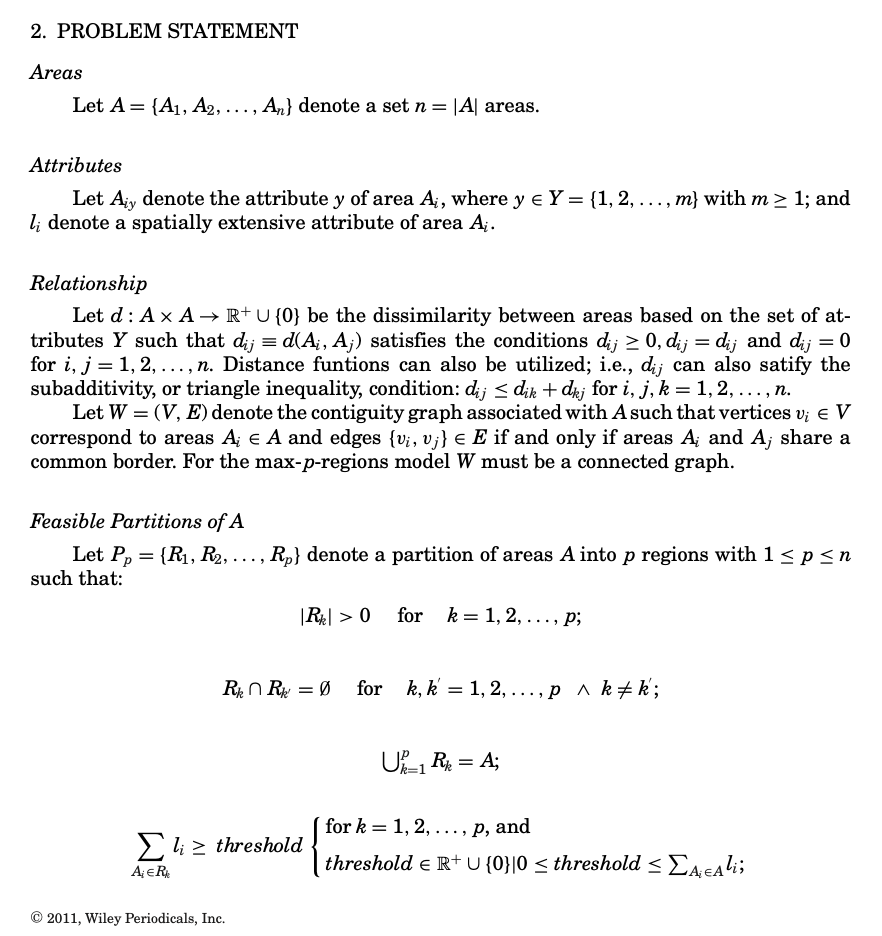
\includegraphics[width=0.70\textwidth]{problem_statement}
  \end{tabular}
\end{center}


\section{Objectives}

\subsection{General objective (\textcolor{red}{sólo uno})}

\begin{comment}
  El objetivo general enmarca todo el trabajo. Está estrechamente relacionado con el
título y con la pregunta de investigación y describe de intensión de la
invesstigación.

La estructura de un objetivo general es la siguiente: verbo en infinitivo (uno
solo) + qué (objeto de estudio) + cómo + para qué.
\end{comment}



\subsection{Specific objectives (\textcolor{red}{3 o 4 objetivos})}

Son un conjunto de objetivos más pequeños que permitirán alcanzar el general.
La estructura de un objetivo general es la siguiente: Verbo en infinitivo (uno
solo) + qué (objeto de estudio) + cómo.

Importante: los objetivos específicos no se pueden confundir con una lista de
tareas. El objetivo debe comenzar con un fin/logro no con el medio/actividad
(las actividades van en la metodología); por ejemplo, un objetivo específico
del tipo ``Realizar una revisión bibliográfica para...'' debería transformarse
en algo como ``Encontrar información científica por medio de una revisión
sistemática de la literatura''.


\section{Justification (\textcolor{red}{4 o 5 párrafos})}

En esta sección se argumenta el por qué es importante resolver el problema o
contestar la pregunta de investigación. Las argumentaciones pueden ser de tipo
teórico o práctico y soportadas en literatura.

\begin{itemize}
\item Destaca los beneficios derivados del aporte (¿para qué servirá esta investigación?, ¿qué aporta de nuevo esta investigación?, ¿cuáles son los beneficios?, ¿quiénes serán los beneficiados y de qué modo?, ¿qué se prevé cambiar con la investigación?, ¿cuál es la utilidad?, ¿resolverá algún problema práctico?, ¿se cubrirá algún gap de conocimiento?, ¿los resultados se podrán generalizar?, ¿sirve para apoyar alguna teoría?, ¿permite un mejor estudio de una población o fenómeno?, ¿se pueden establecer plazos para los beneficios?). OJO: las preguntas no se incluyen en el cuerpo del texto, son sólo una guía para encontrar los argumentos.
\item Las respuestas a estas preguntas deben considerar tres aspectos: teórico, práctico y metodológico.
\end{itemize}


\section{Scope (\textcolor{red}{2 o 3 párrafos})}

Describe las principales barreras o limitaciones de la investigación,
así como las principales herramientas y otros recursos que esperaba utilizar
durante la ejecución del proyecto. También describe los principales
resultados esperados de la investigación

\section{State of the art (\textcolor{red}{5 a 6 párrafos})}

Describe las principales referencias relacionadas con el problema. Este estado
del arte puede referirse al problema o aplicación específica, o bien a los
métodos aplicados para solucionarlo. No debes olvidar incluir los trabajos más
importantes y los más recientes.

\section{Proposed methodology (\textcolor{red}{5 o 6 párrafos})}

Describe en este apartado los métodos, técnicas, algoritmos, etc. que se
utilizarán durante la ejecución del proyecto.

Incluye aspectos como:

\begin{itemize}
\item ¿Qué métodos se suelen usar para responder la pregunta de investigación?
\item ¿Por qué seleccionaste el método que usarás?
\item Describe el método: Supuestos básicos, ventajas y desventajas del método.
\end{itemize}


\section{Schedule, commitments and deliverables}

\begin{itemize}
\item Cronograma de las actividades a realizar durante la PI.
\item Compromisos entre el tutor y el estudiante (e.g., periodicidad de
    reuniones, entrega de datos, etc.).
\item Lista clara de entregables que se esperan de la práctica.
\end{itemize}

Adapta es siguiente cronograma a tu PI.

\begin{table}[h!]
	\begin{center}
     \caption{Schedule}
	\label{tb_sch}
       
    \scalebox{0.78}{
    \normalsize{
		\begin{tabular}{|p{7cm}|r|r|r|r|r|r|r|r|r|r|r|r|r|r|r|r|r|r|}
			\hline
			\multirow{2}{*}{\emph{Activity}} & \multicolumn{18}{c|}{\emph{Weeks}} \\
			\cline{2-19}
            & \emph{\footnotesize 1} & \emph{\footnotesize 2} & \emph{\footnotesize 3} & \emph{\footnotesize 4} & \emph{\footnotesize 5} & \emph{\footnotesize 6} & \emph{\footnotesize 7} & \emph{\footnotesize 8} & \emph{\footnotesize 9} & \emph{\footnotesize 10} & \emph{\footnotesize 11} & \emph{\footnotesize 12} & \emph{\footnotesize 13} & \emph{\footnotesize 14} & \emph{\footnotesize 15} & \emph{\footnotesize 16} & \emph{\footnotesize 17} & \emph{\footnotesize 18} \\
			\hline
			Literature Review & \cellcolor{black}{1}  & \cellcolor{black}{1} & \cellcolor{black}{1} & \cellcolor{black}{1} & \cellcolor{black}{1} &  &  &  &  &  &  &  &  &  &  &  &  &  \\
			\hline
			Research proposal writting & & & &  & \cellcolor{black}{1} & \cellcolor{black}{1} & & & & & & & & & & & & \\
			\hline
			Activity 3 & & & & & & & & & \cellcolor{black}{1} &  \cellcolor{black}{1}& \cellcolor{black}{1} & \cellcolor{black}{1} & & & & & & \\
			\hline
			Results Analysis and comparison & & & & & & & & & & & & & \cellcolor{black}{1} & \cellcolor{black}{1} & \cellcolor{black}{1} & & & \\
			\hline
			Final Report writting & & & & & & & & & & & & & & & & \cellcolor{black}{1} & \cellcolor{black}{1} & \cellcolor{black}{1} \\
			\hline
		\end{tabular}
        }
        }
	\end{center}
\end{table}

\section{Intellectual property}

According to the internal regulation on intellectual property within
Universidad EAFIT, the results of this research practice are product of
\emph{Alejandro Salazar Arango} and \emph{Cristhian David Zambrano Mora}.\\

In case further products, beside academic articles, that could be generated from this work, the intellectual property distribution related to them will be directed under the current regulation of this matter determined by \cite{reglamento2017}.

\bibliographystyle{vancouver}
\bibliography{references.bib}

\end{document}
